\section{Wyzwania}

W związku z nietypowym podejściem do problemu, zarówno projekt, jak i implementacja C-=-1 przedstawiła szereg ciekawych wyzwań.
W szczególności są one powiązane z możliwością wykonywania różnego kodu w zależności od kontekstu uruchomienia oraz publiczną naturą reprezentacji pośredniej.

\subsection{Instancje generyków jako element modelu semantycznego}
Jednym z wyzwań powiązanych z publicznością reprezentacji pośredniej, jest lokalizacja instancji generyków w modelu semantycznym.
Ponieważ generyk 

\begin{figure}
	\caption{Diagram przykładowej relacji pomiędzy pakietami zawierającymi typ generyczny}
	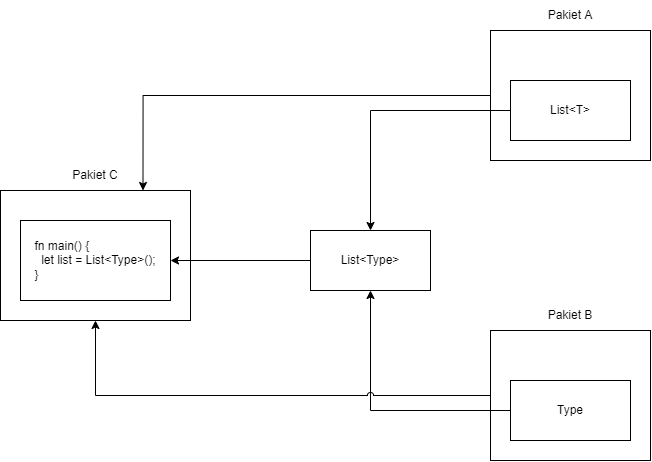
\includegraphics[width=\textwidth]{img/generic_misplaced.png}
\end{figure}

%todo: finish
Gdzie wsadzić instancję generyka?

\subsection{Kod wykonywany w fazie kompilacji}
O tym, czemu atrybuty są przetwarzane przed kodem i nie mogą używać funkcji z biblioteki, w której zostały zdefiniowane.

\subsection{Funkcje generyczne z ograniczeniami}

Funkcje mogą być wykluczane z użycia w trakcie uruchomienia lub kompilacji. Jeśli generyk takiej funkcji zostanie stworzony z typem dalej ograniczającym wykonywalność tej funkcji, ona może być wykonywalna nigdy.

Na wczesnych etapach implementacji, instancje takich generyków były szczególnie problematyczne, ze względu na to jak rozwiązywanie przeciążeń jest zaimplementowane w C-=-1 (rozdział \ref{Function_overload_resolution}).
W związku z tym, w wypadku użycia funkcji generycznej, kompilator powołuje instancje wszystkich wersji tego szablonu, ze zgodną ilością parametrów.
Niektóre z nich, mogą być niepoprawne w danym kontekście. 

Na przykład operator \lstinline{new unique} został zdefiniowany w dwóch wersjach: na czas uruchomienia oraz kompilacji.
W czasie uruchomienia, odwołuje się on do funckji \lstinline{unsafe_new} która alokuje zadaną ilość bajtów na stercie.
W czasie kompilacji wywołuje funkcję generyczną \lstinline{compiletime_heap_allocate} która zwraca referencję na instancję zadanego typu.
Szczegóły zostały opisane w rozdziale \ref{operator_new}.

Sygnatury tych operatorów niczym się nie różnią.
Język rozpoznaje je jako oddzielne, rozróżnialne byty wyłącznie dlatego, że atrybuty którymi został adnotowane zmieniają ich dostępność w czasie kompilacji i uruchomienia.

Na wczesnych etapach implementacji, instancje funkcji generycznych były tworzone, przy założeniu że ich kod będzie poprawny semantycznie.
Takie samo założenie obowiązuje przy tworzeniu zwykłych funkcji, ponieważ ze względu na ograniczenia czasowe, raportowanie o błędach kompilacji nie jest częścią pracy.
Kompilator najpierw kompletował reprezentacje pośrednią instancji wszystkich wersji generyków pasujących do danego użycia.
Przy próbie dynamicznej alokacji typu który nie mógł istnieć w czasie uruchomienia, takiego jak deskryptor funkcji, prowadziło to do odrzucenia poprawnego programu.

Naprawa tego problemu, wymagała weryfikacji czy dana funkcja jest wykonywalna, w jakimkolwiek kontekście, po wykonaniu kodu powiązanych atrybutów.
Alternatywnym podejściem jest ignorowanie traktowanie błędów w instancji generyka, jako sygnał do odrzucenia tej specjalizacji, tak jak zostało to rozwiązane w C++ \cite{cppTemplatesCompleteGuide}.
Takie rozwiązanie mogłoby jednak prowadzić do zaśmiecania modelu semantycznego funkcjami, które nie mogą zostać użyte w żadnym kontekście i nie zawierały akurat żadnych błędów.
%todo: formalize?
\subsection{Operator new}
\label{operator_new}
Operator \lstinline{new} w C-=-1, tak jak w C++ służy do dynamicznej alokacji pamięci na stercie.

\subsection{Wybór przeciążenia funkcji}
\label{Function_overload_resolution}
To czy funkcja jest wykonywalna w czasie kompilacji albo uruchomienia można ustalić bardzo późno w trakcie budowy modelu semantycznego.

Na pytanie "czy ta funkcja może być użyta w tym kontekście", kompilator jest w stanie odpowiedzieć dopiero kiedy wykonanły się na niej funkcje \lstinline{attach} wszystkich powiązanych z nią atrybutów.

%todo: example?

\subsection{Wyrażenia literałowe}

Wyrażenie literałowe przedstawia stałą wartość.
Na przykład w języku C++ \lstinline{int a = 4;} deklaruje i inicjalizuje zmienną a literałem 4.
Wyrażenia lietrałowe mogą reprezentować stałe różnych typów wbudowanych.

\subsection{Integracja z back-endem}
\label{backend_integration}
Przy pierwszym podejściu do budowy reprezentacji pośredniej, użyto dedykowanych struktur danych. Było to podejście najbardziej naturalne i dające najwięcej bezpieczeństwa dzięki silnemu typowaniu. Wszystkie struktury danych opisane w rozdziale \ref{reprezentacja_posrednia} miały powiązane ze sobą klasy C++.


To podejście tworzy jednak duży problem. Reprezentacja pośrednia musi zostać wyeksponowana użytkownikowi. Ponieważ nie istniała możliwość stworzenia binarnego interfejsu między kompilatorem a interpretowanym kodem, struktury danych CIR musiały być dodatkowo reprezentowane za pomocą struktur danych interpretera.


Użytkownik może dokonywać modyfikacji w CIR, co oznacza że może dojść do rozbieżności między strukturami danych interpretera a kompilatora. Utrzymywanie tych dwóch reprezentacji stanowiło poważne wyzwanie, dlatego postanowiono zmienić podejście. Użycie wyłącznie struktur danych interpretera do reprezentacji CIR usunęło ten problem, kosztem bezpieczeństwa kodu.


Ponieważ w nowym podejściu, z perspektywy C++ niemalże wszystkie obiekty miały ten sam typ, kompilator stracił możliwość statycznej weryfikacji kodu.
Aby zapewnić poprawność programu, koniecznym stało się dodawanie analizy argumentów do wszystkich funkcji.
